\subsection{Reflections and amplitude damping}

In section \ref{gbh} the wave behavior of the voltage and current is discovered. To this end, the analysis of voltage waves at the boundaries for specific values of the generator resistance $R_g$ and load resistance $R_L$ is discussed. We highly recommend watching the simulation \href{https://ugentbe-my.sharepoint.com/:f:/g/personal/constantijn_coppers_ugent_be/Evlx5Q0EKRhCggn-R1x3NKQBhiF82wRowFP4pT1nCn1ymg?e=Xi2V3R}{video's}\footnote{Simulation details and visualizations are stored in a OneDrive. Only accessible for UGhent members.\label{fn}}. \\

Our first question concerns the entrance of the bit to the transmission line (TL): the simulation starts at $t=0$ and the generator $\hat{e}_g$ produces a bit with amplitude $V_0$. Before the bit enters the TL, it meets the generator resistance $R_g$ and thus energy will be dissipated i.e. the voltage amplitude is dampened. This can be clarified by expressing Kirchoff's Voltage Law at the origin ($z=0$) of the TL;

\begin{align}
&\hat{e}_g(t) = (R_g + R_c)\hat{i}(0, t) \\
&\Rightarrow \hat{i}(0, t) = \frac{1}{R_g+R_c}\hat{e}_g(t)= \frac{1}{R_c}(\hat{v}^{+}(0, t) - \hat{v}^{-}(0, t)) \\
&\Rightarrow \hat{v}(0, t) = \hat{v}^{+}(0, t) =\kappa\hat{e}_g(0, t)\label{enter}.
\end{align}
The amplitude $V_0$ of the generated bit is reduced by a factor $\kappa = \frac{R_c}{R_g + R_c}$. Here, the role of the characteristic impedance becomes clear; at the beginning of the TL, the bit 'sees' it as input impedance, but does not dissipate energy to it; the bit amplitude remains constant during its passage through the TL. Indeed, the TL is lossless and only contains p.u.l capacitances and inductances (passive). One can observe two interesting cases:
\begin{itemize}
\item $R_g = 0 \Rightarrow \kappa = 1$\\ The generated bit freely enters the TL since it does not meet resistance.
\item $R_g = \infty \Rightarrow \kappa = 0$ \\ The circuit is open. The bit can not enter the TL.
\end{itemize}

Now, assume the bit is able to enter the transmission line ($R_g \neq \infty$) and propagates lossless towards the load with, obviously, constant speed $c$. Again, at the load ($z=d$), Kirchoff's Voltage Law must be satisfied. Consequently, a reflected wave with lower or equal amplitude will be originated (Figure \ref{fig:refl});
\begin{align}
&\hat{v}(d, t) = \hat{v}^{+}(d, t) + \hat{v}^{-}(d, t) = R_L\hat{i}(d, t) \\
&\Leftrightarrow \hat{v}^{+}(d, t) + \hat{v}^{-}(d, t) = \frac{R_L}{R_c}(\hat{v}^{+}(d, t) - \hat{v}^{-}(d, t)) \\
&\Leftrightarrow (1 + K_L)\hat{v}^{+}(d, t) = \frac{R_L}{R_c}(1 - K_L)\hat{v}^{+}(d, t) \\
&\Rightarrow K_L = \frac{R_L/R_c - 1}{R_L/R_c + 1} = \frac{R_L - R_c}{R_c + R_L}.
\end{align}


$K_L$ is also know as the reflection coefficient at the load. This constant determines how much of the amplitude is reflected back:
\begin{enumerate}
\item $R_L > R_c \Rightarrow K_L > 0$ \label{ref1} (Figure \ref{fig:damp} A) \\
	The voltage wave arriving at the load does not have enough power. Since the load impedance is not matched with the characteristic impedance, the voltage at the load must take the load impedance into account (KCL); the net voltage $\hat{v}$ is compensated such that its amplitude at the load is higher than the amplitude of the wave arriving at $R_L$; a backward wave is originated that satisfies $\hat{v}^{-} = K_L\hat{v}^{+}$, because than $$\hat{v}(d, t) = (1 + K_L)\hat{v}^{+}(d, t).$$ This might be counterintuitive, since one might think it violates the law of conservation of energy. Luckily, this is not true; comparing the input power to the power delivered to the load (first reflection) gives
	\begin{align}
		&P_{\text{in}} > P_L \\
		&\Leftrightarrow \frac{\kappa^2 V^2_0}{R_c} > \frac{(1 + K_L)^2\kappa^2V^2_0}{R_L} \\
		&\Leftrightarrow (R_L-R_c)^2 > 0 \label{Pw}.
	\end{align}
Equation (\ref{Pw}) is always true and the law of conservation of energy still holds. The reflected wave still contains $P_{\text{in}} - P_L$ power.
\item $R_L = R_c \Rightarrow K_L = 0$: matching (Figure \ref{fig:damp} B,  \href{https://ugentbe-my.sharepoint.com/:f:/g/personal/constantijn_coppers_ugent_be/Evlx5Q0EKRhCggn-R1x3NKQBhiF82wRowFP4pT1nCn1ymg?e=Xi2V3R}{video matching})\\
	From an engineering point of view, this is the most wanted; the energy of the forward wave is fully dissipated to the load. Maximum power is reached and there is no reflection back.
	
\item $R_L < R_c \Rightarrow K_L <0$ \\
	The same principle holds as in case \ref{ref1}, with the difference that the reflected wave amplitude has an opposite sign compared to the incident wave; that is, because the voltage wave arriving at the load contains too much energy.

\item $R_L \longrightarrow \infty \Rightarrow K_L \longrightarrow 1$ \\
	The electric circuit is open. When the voltage wave arrives at the end of the TL, it is fully reflected to the load and no energy is dissipated.
	
\end{enumerate}
Obviously, when the reflected wave arrives back at the generator it might be reflected back to the load, depending on the value of the generator impedance. In summary, the generated bit enters the TL weakened (\ref{enter}) and starts to move back and forth between the load impedance and generator impedance, whereby energy is dissipated and the amplitude reduces until the wave is fully dampened (\href{https://ugentbe-my.sharepoint.com/:f:/g/personal/constantijn_coppers_ugent_be/Evlx5Q0EKRhCggn-R1x3NKQBhiF82wRowFP4pT1nCn1ymg?e=Xi2V3R}{video amplitude damping}$^{\ref{fn}}$).

\begin{figure}[h!]
\centering
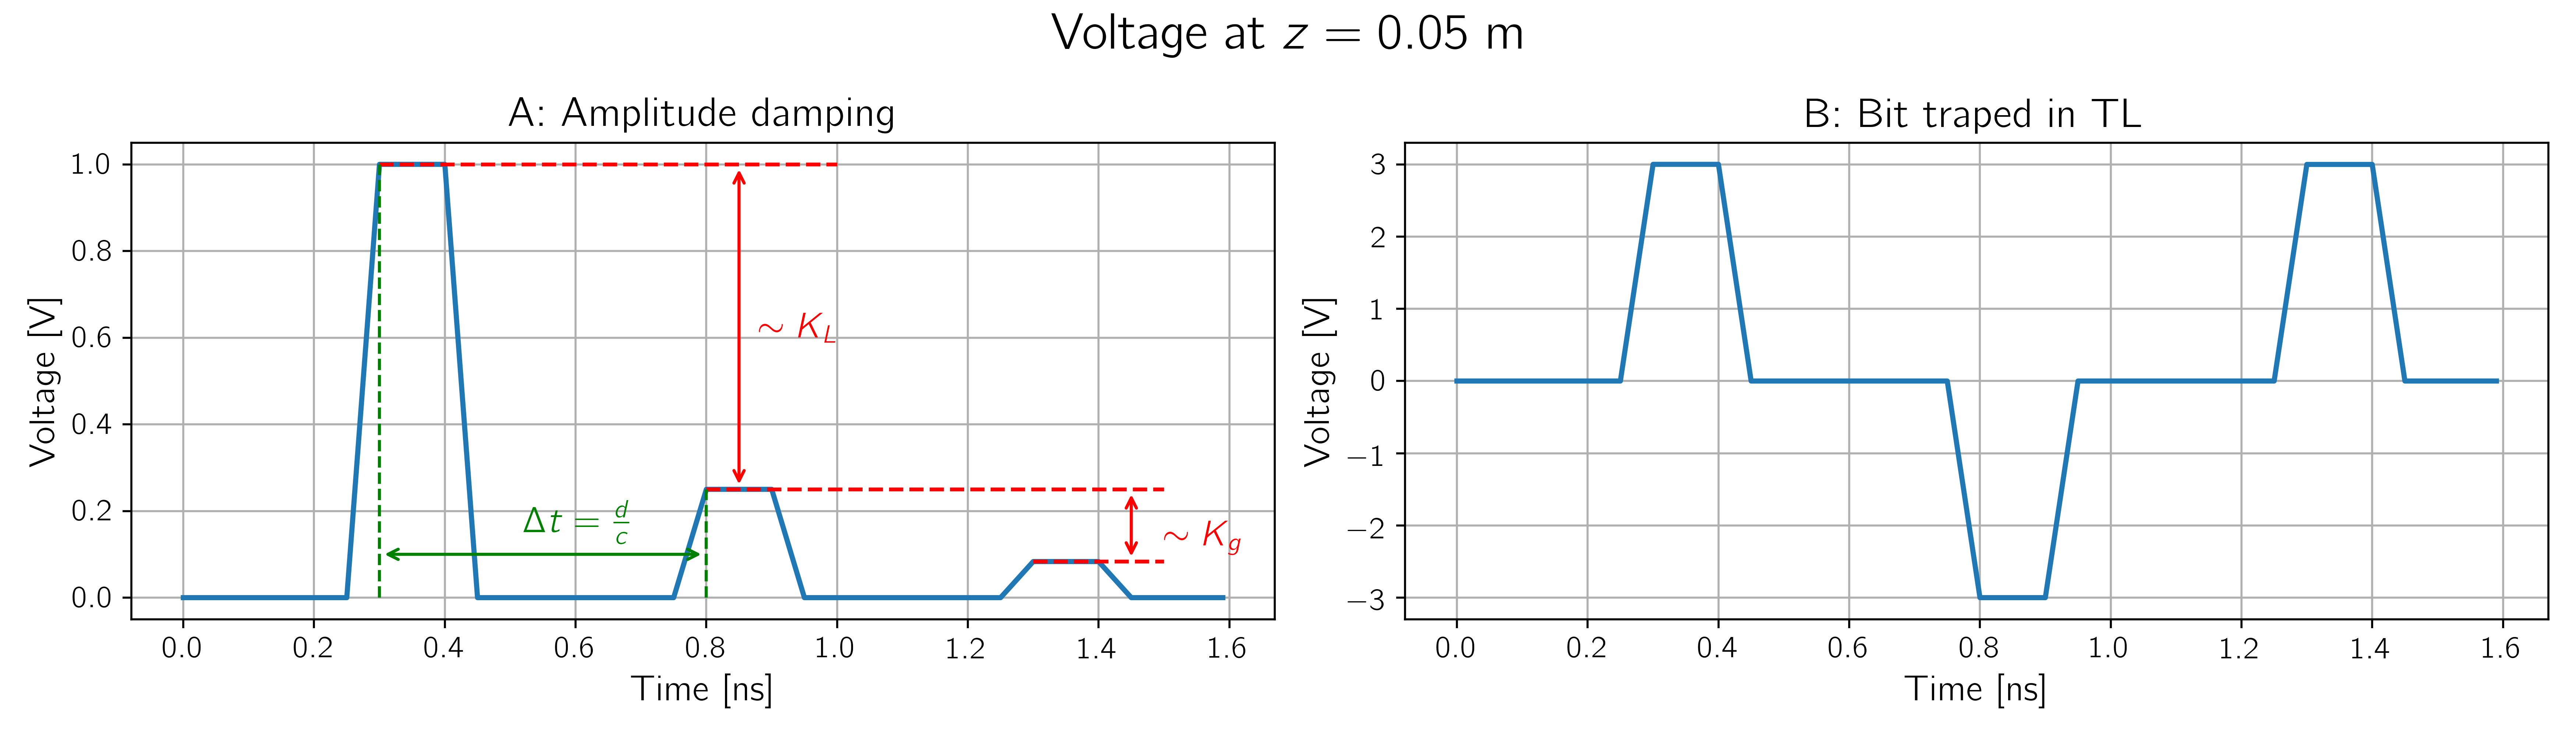
\includegraphics[width = \textwidth]{amplitudeplot.png}
\caption{FDTD simulations of a voltage wave traveling trough a TL. This wave moves with constant speed $c$ and is reflected at the load- and generator impedance with a damping factor $K_L$ resp. $K_g$. In A, the bit amplitude decreases as it meets an impedance. In B, the bit is trapped in the TL ($K_L\approx-1$ and $K_g \approx1$).}\label{fig:damp}
\end{figure}

\begin{figure}[h!]
\centering
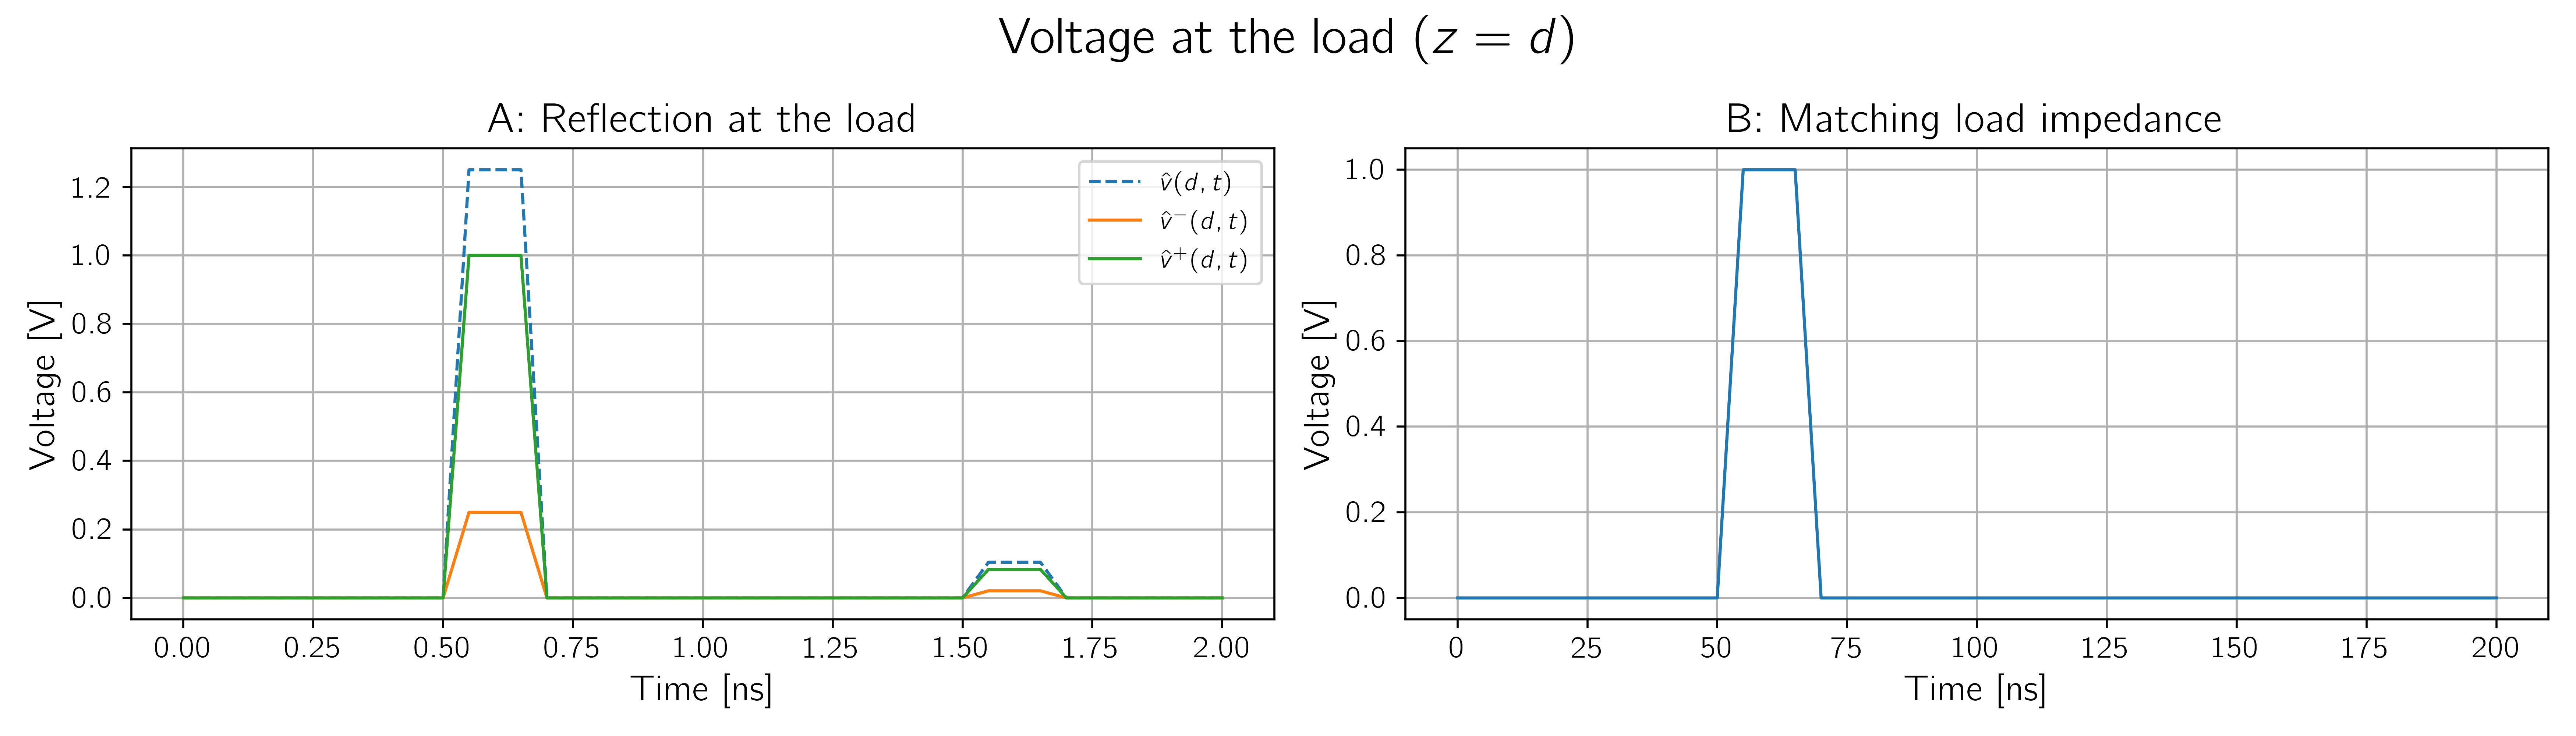
\includegraphics[width = \textwidth]{reflection.png}
\caption{Plot of voltage wave (FDTD simulation) at the load and decomposed into its forward $\hat{v}^{+}$ and backward $\hat{v}^{-}$ component.}\label{fig:refl}
\end{figure}